\subsection{Fuentes de campos magnéticos}

Anteriormente probablemente haya visto que partículas con masa generan un campo gravitatorio y pueden interactuar con otros campos gravitatorios. También que cargas eléctricas generan un campo eléctrico y pueden interactuar con otros campos eléctricos. Para las cargas en movimiento no es la excepción, tal y como las otras interacciones, las cargas en movimiento interactúan con campos magnéticos y generan campos magnéticos.

Antes de continuar es importante aclarar un detalle importante en la analogía de arriba. Que un objeto con masa genere un campo gravitatorio \textbf{no} significa que los campos gravitatorios interactuen entre sí. Lo mismo para los campos eléctricos y magnéticos. La interacción no es campo-campo, sino más bien \textit{objeto-campo}. En el caso del campo magnético la interacción ocurre entre una carga en movimiento y un campo magnético, o entre una corriente y un campo magnético.

\subsubsection{Campo magnético de una carga en movimiento}

Para poder explicarlo veamos la figura \ref{fig:lineas_de_campo_magnético_de_la_carga_puntual}. En esta figura se muestran las líneas de campo magnético generadas por una carga puntual que se mueve con velocidad constante.

\begin{figure}[ht]
  \centering
  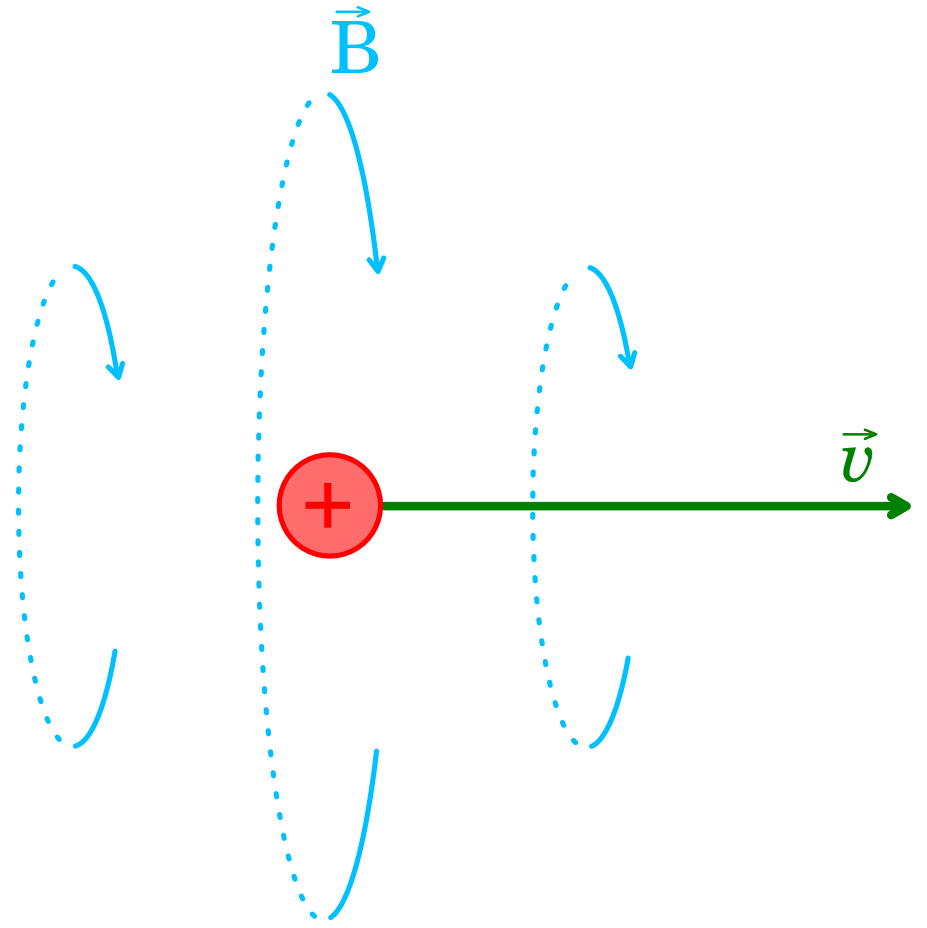
\includegraphics[width=0.3\textwidth]{squematic_charge_magnetic_field.png}
  \caption{Líneas de campo magnético de la carga puntual.}
  \label{fig:lineas_de_campo_magnético_de_la_carga_puntual}
\end{figure}

El campo magnético \(\vec{B}\) generado por la carga puntual \(q\) que se mueve con velocidad constante \(\vec{v}\) en \textbf{un punto del espacio} \(\vec{r}\) está dado por:

\begin{equation}
  \vec{B} = \frac{\mu_0}{4\pi} \frac{q \, \vec{v} \times \hat{r}}{r^2}
  \label{eq:campo_magnético_de_una_carga_puntual}
\end{equation}
donde:
\begin{itemize}
  \item \(\mu_0 = 4 \pi \times 10^{-7} \, \frac{\si{\newton}}{\si{\ampere\squared}}\) es la permeabilidad del vacío,
  \item \(\vec{r}\) es el vector que apunta desde la posición de la carga al punto donde se evalúa el campo,
  \item \(r = |\vec{r}|\) es la magnitud del vector \(\vec{r}\),
  \item \(\hat{r} = \frac{\vec{r}}{r}\) es el vector unitario en la dirección de \(\vec{r}\).
\end{itemize}

\begin{wrapfigure}{r}{0.3\textwidth}
  \centering
  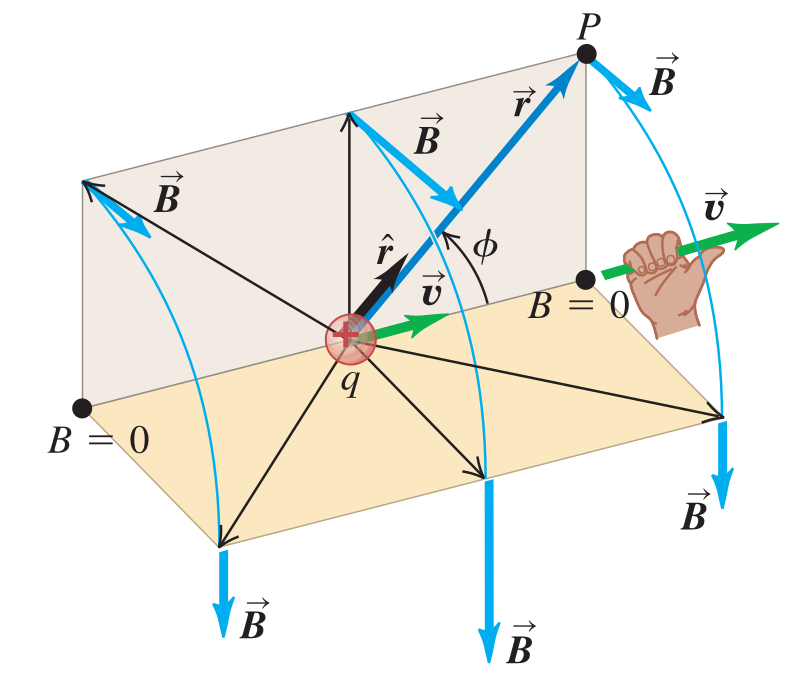
\includegraphics[width=\linewidth]{magnetic_field_of_a_point_charge.png}
  \caption{Campo magnético de una carga puntual.}
  \label{fig:campo_magnético_de_una_carga_puntual}
\end{wrapfigure}
La forma del campo magnético generado por \(q\) es circular, y \(\vec{B}\) es perpendicular a \(\vec{v}\) y \(\vec{r}\). Como se muestra en la figura \ref{fig:campo_magnético_de_una_carga_puntual} el campo magnético \(\vec{B}\) decrece con la distancia al punto \(P\). Además mientras menor es el ángulo entre \(\vec{v}\) y \(\vec{r}\) menor será el campo magnético \(\vec{B}\), y en el caso particular de \(\theta = 0^\circ\) el campo magnético \(\vec{B}\) será cero. 

Este campo magnético es el responsable de que las cargas en movimiento experimenten una fuerza magnética \(\vec{F}_B = q\vec{v} \times \vec{B}\).

Es importante recordar que \textbf{las líneas de campo magnético siempre son cerradas}. Esto lo vimos en la sección \ref{sec:flujo_magnético}, si encerramos un imán en una superficie Gaussiana, todas las líneas de campo magnético que salen, vuelven a entrar. Esto resulta en un flujo nulo.

\begin{tcolorbox}[myconclusion]
  El campo magnético total generado por varias cargas en movimiento es la suma vectorial de los campos generados por las cargas individuales.
\end{tcolorbox}

Con esto en mente, podemos encontrar el campo magnético generado por un diferencial de carga. De la sección \ref{sec:movimiento_de_cargas} sabemos que para un pedacito de segmento de longitud \(dl\) la carga es:
\[
dq = nqA\, dl
\]

De la ecuación \ref{eq:campo_magnético_de_una_carga_puntual} podemos aplicar la definición geométrica del producto vectorial, y reemplazar la carga por la expresión anterior. Entonces el campo magnético \(dB\) generado por un diferencial de carga es:
\begin{align*}
  dB &= \frac{\mu_0}{4\pi} \frac{dq \, v_d \, \sin\theta}{r^2} \\
  dB &= \frac{\mu_0}{4\pi} \frac{\left(nq v_d A\right) dl}{r^2} \sin\theta \\ 
  dB &= \frac{\mu_0}{4\pi} \frac{I dl}{r^2} \sin\theta 
\end{align*}

Entonces el un diferencial de campo magnético \(d\vec{B}\) generado por una corriente \(I\) que fluye a través de un pequeño segmento \(dl\) es:
\begin{equation}
  \boxed{d\vec{B} = \frac{\mu_0}{4\pi} \frac{I \, d\vec{l} \times \hat{r}}{r^2}}
  \label{eq:campo_magnetico_de_un_diferencial_de_corriente}
\end{equation}

\subsubsection{Ley de Biot-Savart}

La fórmula \ref{eq:campo_magnético_de_una_carga_puntual} es una versión simplificada de la Ley de Biot-Savart para una carga puntual. A partir de \eqref{eq:campo_magnetico_de_un_diferencial_de_corriente} podemos obtener la Ley de Biot-Savart que establece que el campo magnético \(\vec{B}\) generado por una corriente \(I\) que fluye a través de una curva \(C\) es:

\begin{equation}
  \vec{B} = \frac{\mu_0}{4\pi} \int_C \frac{I \, \vec{dl} \times \hat{r}}{r^2},
\end{equation}
donde:
\begin{itemize}
  \item \(\mu_0 = 4 \pi \times 10^{-7} \, \frac{\si{\newton}}{\si{\ampere\squared}}\) es la permeabilidad del vacío,
  \item \(\vec{dl}\) es el vector diferencial de longitud de la curva \(C\),
  \item \(r = |\vec{r}|\) es la magnitud del vector \(\vec{r}\),
  \item \(\hat{r} = \frac{\vec{r}}{r}\) es el vector unitario en la dirección de \(\vec{r}\).
\end{itemize}

\subsubsection{Aplicación de la ley de Biot-Savart}

La ley de Biot-Savart es una ecuación general que describe el campo magnético generado por una corriente. Sin embargo, en la práctica, su aplicación puede ser compleja, especialmente cuando se trata de curvas complejas o cuando se requiere resolver integrales complejas.

En la aplicación práctica de la ley de Biot-Savart, es común simplificar la integración considerando curvas rectas o cilíndricas, lo que permite resolver integrales más simples. Incluso es posible determinar la dirección del campo magnético con la regla de la mano derecha y calcular únicamente el módulo del campo magnético. A continuación se dan los resultados de algunos de los casos más comunes.

Para un segmento largo y recto de cable el módulo del campo magnético se convierte en:
\begin{equation*}
  B = \frac{\mu_0 I}{2\pi r}
\end{equation*}
donde:
\begin{itemize}
  \item \(\mu_0 = 4 \pi \times 10^{-7}\) es la permeabilidad del vacío,
  \item \(I\) es la corriente que fluye a través del cable,
  \item \(r\) es la distancia desde el cable al punto donde se evalúa el campo magnético.
\end{itemize}

\noindent Para una espira circular de radio \(R\) el módulo del campo magnético en el centro es:
\begin{equation*}
  B = \frac{\mu_0 I}{2R}
\end{equation*}

\noindent Para un solenoide de N espiras de radio \(R\) el campo en el centro es:
\begin{equation*}
  B = \mu_0 \frac{N I}{2R}
\end{equation*}